%==============================================================================
\FloatBarrier
%------------------------------------------------------------------------------
\section{Raster plots}
\label{sec:pl_rasters}

Here's some exemplar raster plots.


%------------------------------------------------------------------------------
\section{Stimulus response curves}
\label{sec:pl_response_curves}
%------------------------------------------------------------------------------

Here's some exemplar response curves.

\begin{figure}[htbp]
    \centering
    \hspace*{\fill}
    \subfloat[\ac{M1} \ac{V1}\label{fig:respcurve_v1_blanco}]{
        \centering
        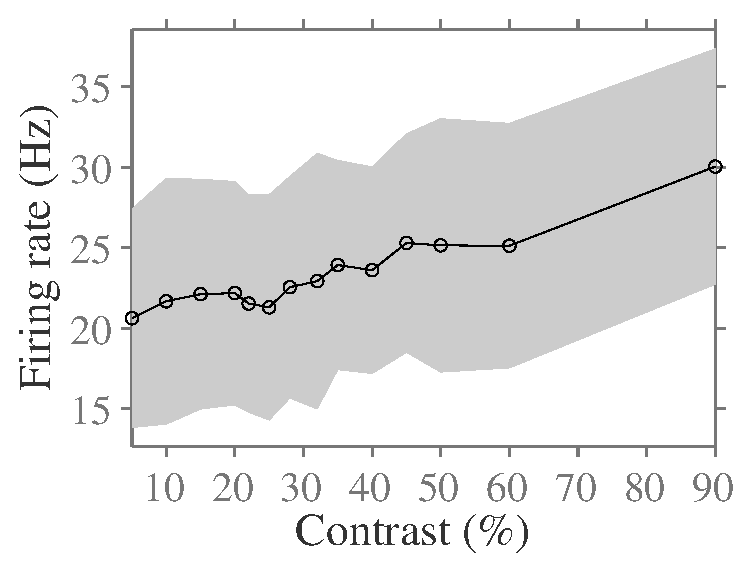
\includegraphics[scale=.45]{%
figs/response_curve/respcurve_blanco_v1_ch11_s359.eps}
    }
    \hspace{.4cm}
    \subfloat[\ac{M2} \ac{V1}\label{fig:respcurve_v1_jack}]{
        \centering
        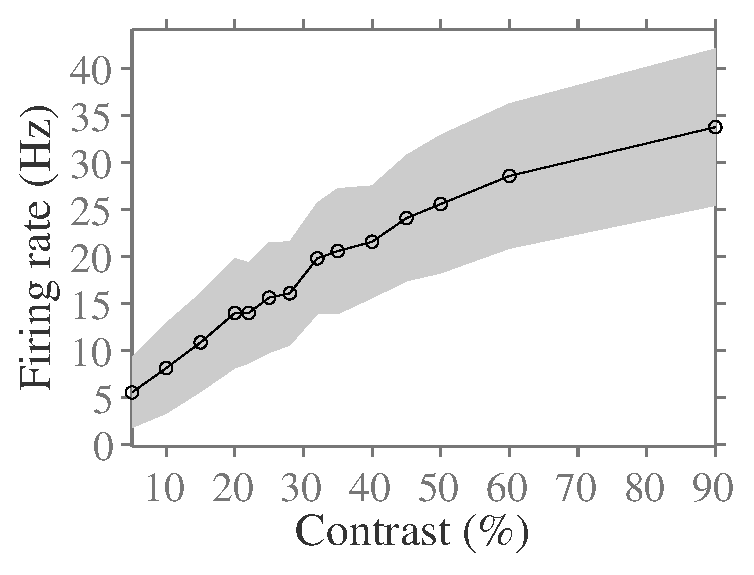
\includegraphics[scale=.45]{%
figs/response_curve/respcurve_jack_v1_ch12_s72.eps}
    }
    \hspace*{\fill}
    \\
    \hspace*{\fill}
    \subfloat[\ac{M1} \ac{V4}\label{fig:respcurve_v4_blanco}]{
        \centering
        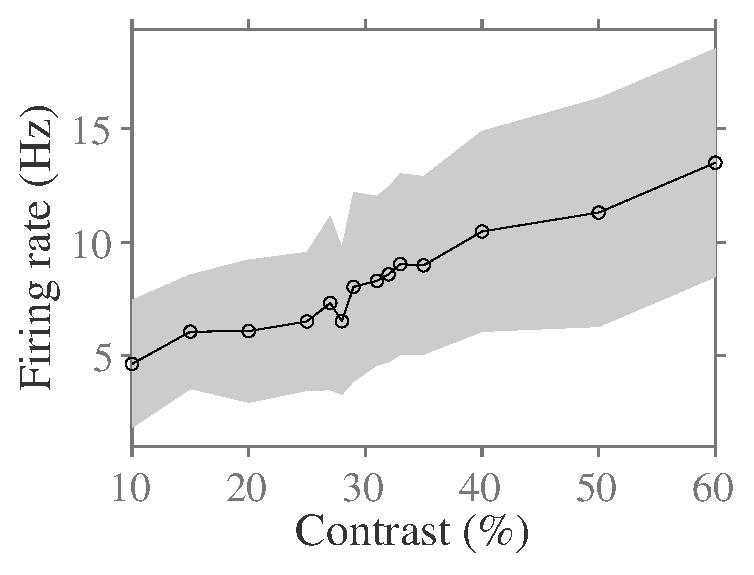
\includegraphics[scale=.45]{%
figs/response_curve/respcurve_blanco_v4_ch51_s341.eps}
    }
    \hspace{.4cm}
    \subfloat[\ac{M2} \ac{V4}\label{fig:respcurve_v4_jack}]{
        \centering
        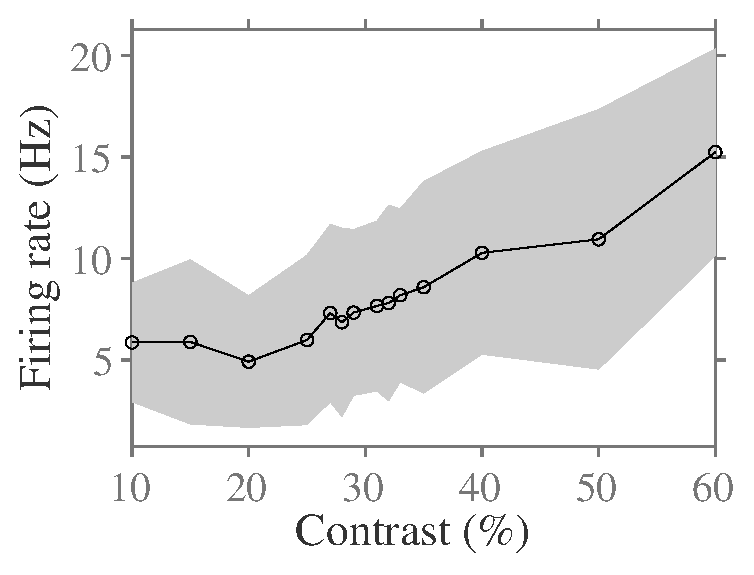
\includegraphics[scale=.45]{%
figs/response_curve/respcurve_jack_v4_ch6_s49.eps}
    }
    \hspace*{\fill}
    \caption{Stimulus response curve.
}
    \label{fig:respcurve}
\end{figure}
